
\chapter{Introduction}


Cancer is a complex and heterogeneous disease that arises from a combination of genetic and environmental factors. According to the International Agency for Research on Cancer (IARC)\footnote{\url{https://www.iarc.who.int/}}, approximately one in five individuals worldwide develop cancer during their lifetime. Unfortunately, the incidence and mortality of cancer are rapidly increasing \cite{CAtoday}, with the GLOBOCAN 2020 projecting 28.4 million new cases of cancer globally by 2040, which represents a 47\% increase from 2020 \cite{bray2018global}. Moreover, cancer is a leading cause of deaths across the globe, accounting for nearly 10 million deaths in 2020. A recent study showed that cancer was the first or second cause of premature death (\ie under the age of 70) in 112 of 183 countries analyzed, and ranked third or fourth in other 23 countries \cite{CAtoday}, as shown in Figure~\ref{fig:cancermortality}. Thus, early detection and treatment of cancer lesions are crucial in reducing cancer mortality rates and the burden of this major public health problem.

\begin{figure}[!h]
    \centering
      \caption{National ranking of cancer as a cause of premature death in 2019.}
    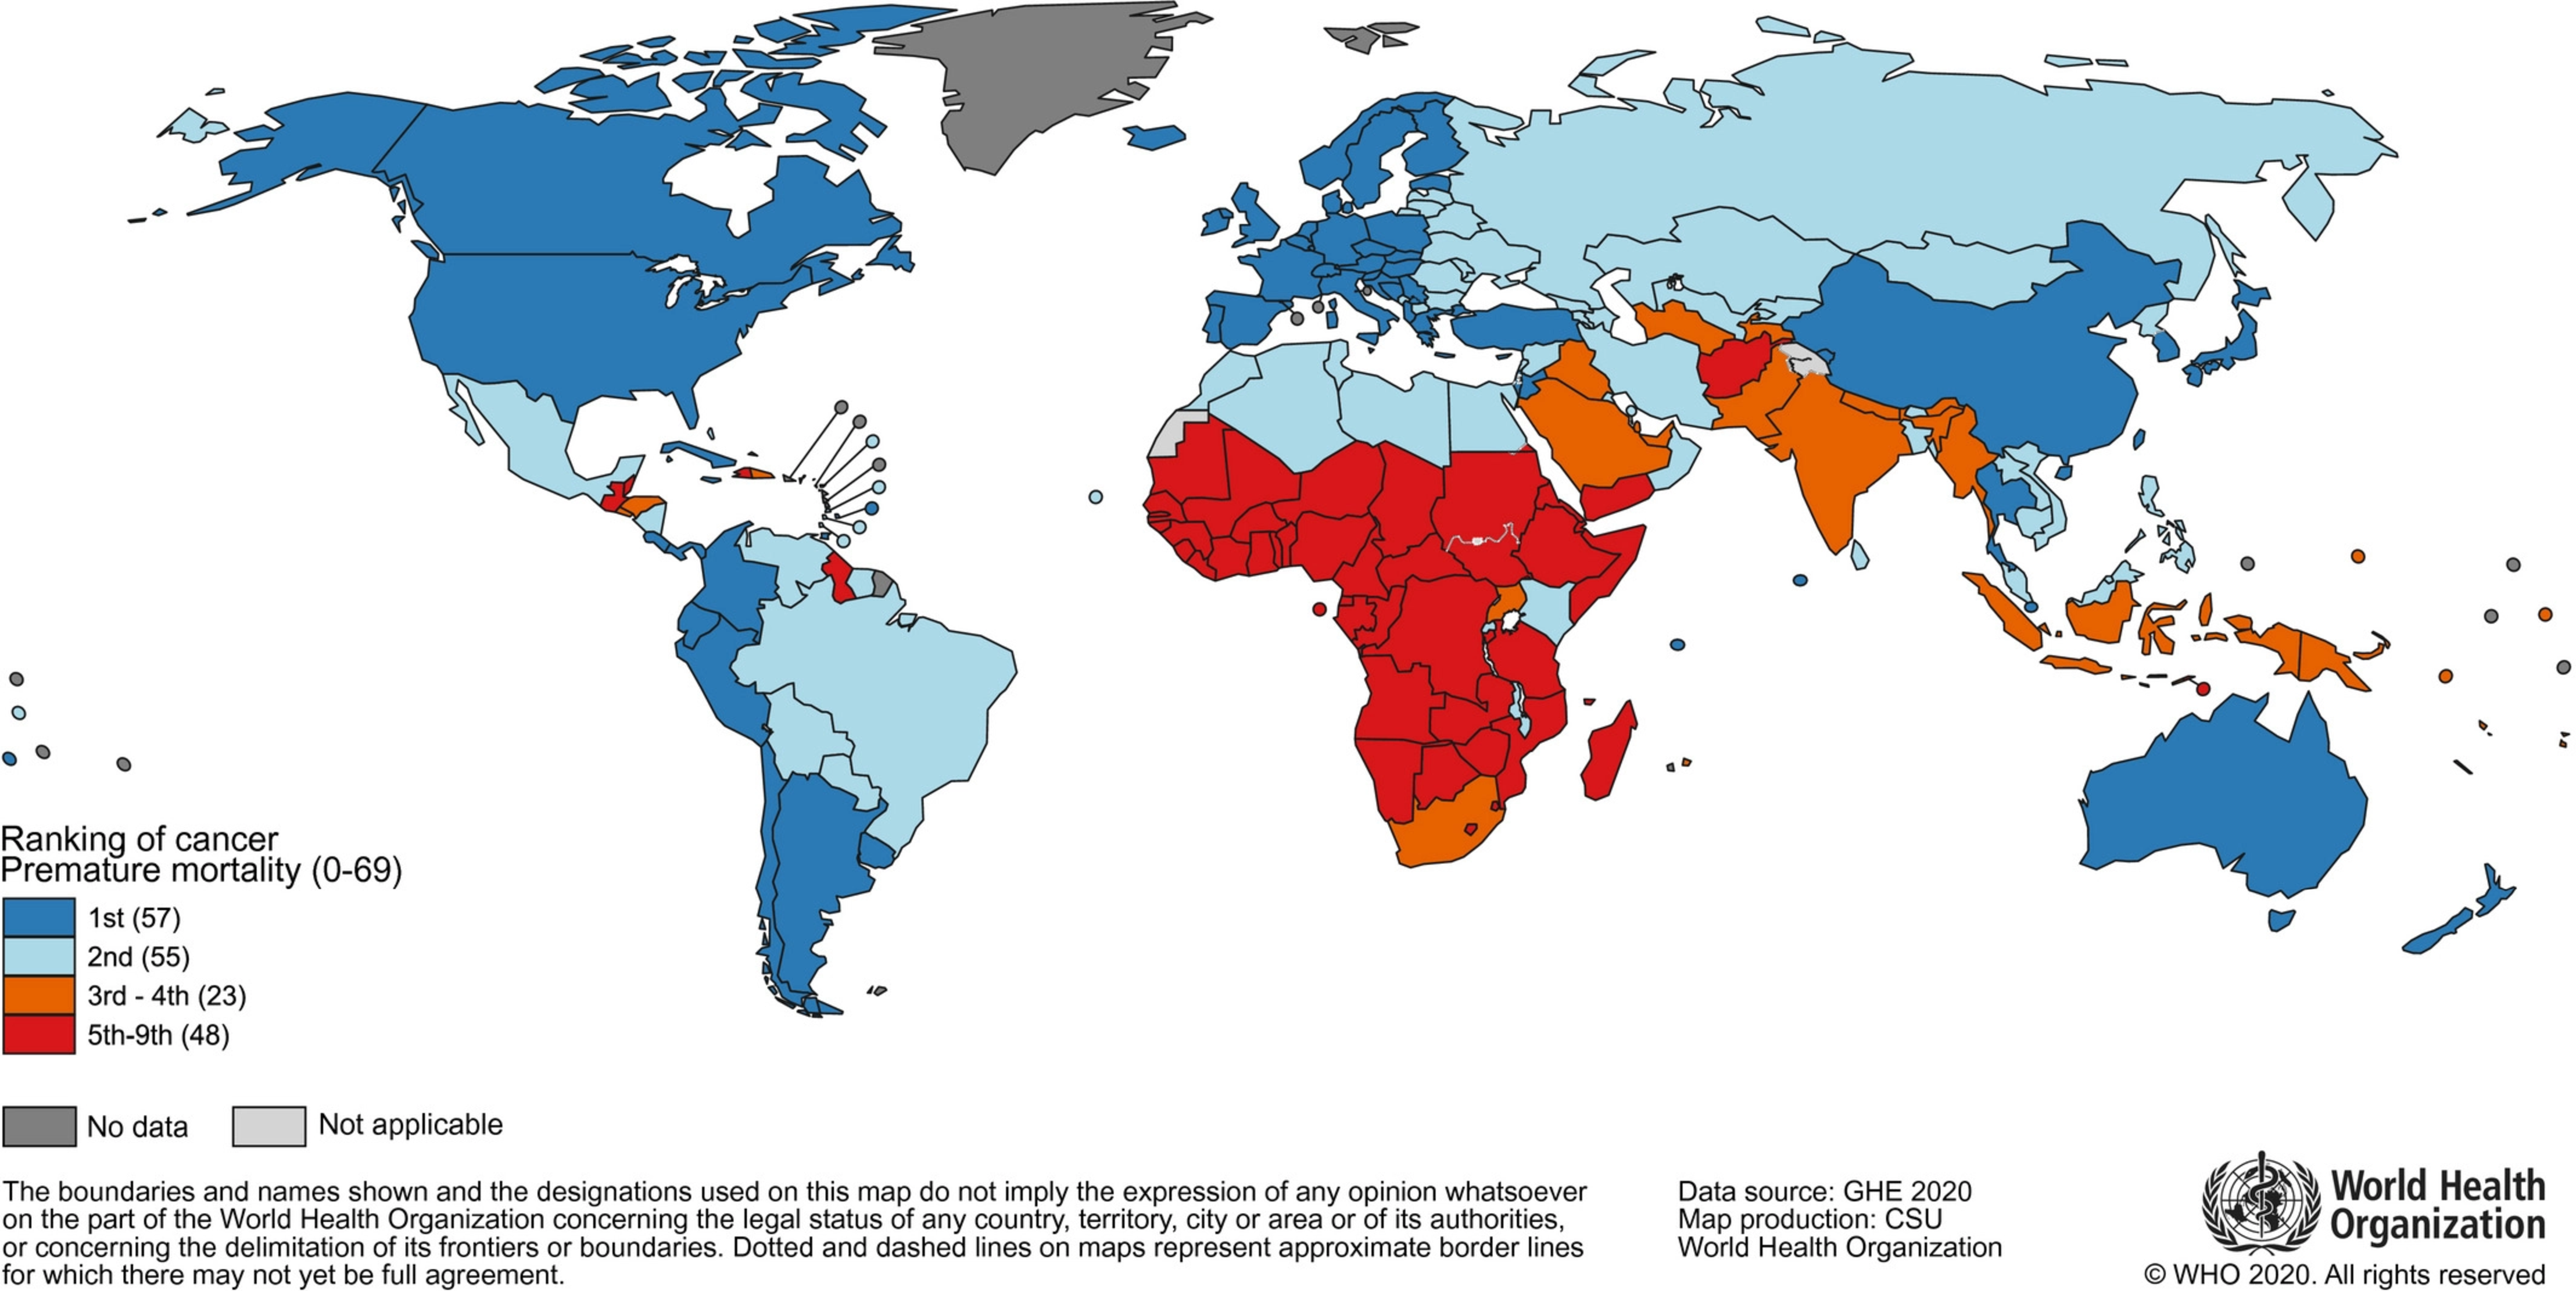
\includegraphics[width=0.95\textwidth]{images/ilustracoes/cancer_mortality.pdf}
    \legend{Source: \citet{CAtoday}}
    \label{fig:cancermortality}
\end{figure}

As a multifactorial disease, several factors may impact cancer risk. The risk factors include environmental and lifestyle factors, such as UV radiation, air pollution, cigarette smoking, hormone therapy, physical activity, and dietary patterns \cite{wu2018evaluating}. Nonetheless, cancer is largely the result of acquired genetic and epigenetic changes that culminate in abnormal and uncontrolled cell growth \cite{tomasetti2015variation,anandakrishnan2019estimating}. Somatic mutations, which are genetic alterations acquired during an individual's lifetime, are the most significant contributors to tumorigenesis \cite{martinez2020compendium}. Specifically, the somatic mutations that confer a selective growth advantage to a tumor cell, called ``driver'' mutations, reside in a subset of genes known as cancer driver genes (CDGs) \cite{stratton2009cancer}. However, the majority of somatic mutations are neutral or ``passenger''  mutations that have no impact on cancer initiation and progression \cite{stratton2009cancer, vogelstein2013cancer}. Thus, identifying all genes carrying mutations that can drive carcinogenesis is a major goal in cancer research. 

Distinguishing between driver mutations and passenger mutations is a challenging task, despite the increasing availability of cancer genomic datasets. The heterogeneity of mutation rate and mutation types across tumors pose the need for rigorous analytical methods that can effectively deal with these issues and also handle the natural challenges of genomic data analysis  \cite{martinez2020compendium}. Various computational approaches have been proposed to improve the detection of driver mutations and CDGs from genomics data. Machine learning (ML) algorithms have been particularly successful in predicting CDGs, as noted in a recent survey \cite{andrades2022machine}. However, advanced deep learning (DL) techniques are gaining momentum in the field by enabling the construction of end-to-end models that can handle complex data. 

Among DL methods, there has been a growing interest in the use of graph-based learning algorithms for prediction tasks in bioinformatics due to their ability to learn patterns from graph-structured data modeling the complex relationship and manifold interactions among biological entities \cite{georgousis2021graph}. Specifically, graph neural networks (GNN) are emerging as key tools since they have shown promise in learning in the presence of irregular geometric shapes commonly found in biology, such as in protein-protein interaction (PPI) networks. Moreover, these algorithms allow integrating node-level features into the learning process, creating rich node embeddings that encompass information from nodes' properties and local structure in the graph.


However, there is limited exploration of GNNs for predicting CDGs across different cancer types. Existing research has shown the potential of GNNs to integrate PPI networks and high-throughput omics data, such as transcriptomic and epigenetic data from healthy and tumor tissues, to identify CDGs more accurately \cite{Schulte-Sasse2019, schulte2021integration}. Nevertheless, several data-centric strategies in GNN-based models' development, such as node feature vectors, node centrality measures, and class imbalance mitigation methods, remain unexplored. Additionally, previous works have not investigated the concept of ensemble learning alongside GNNs for CDGs prediction. Therefore, further research is needed to determine the effectiveness of these strategies in improving CDGs prediction.

In light of this, the present study aims to propose an effective approach for predicting cancer driver genes (CDGs) by exploring graph neural network (GNN) algorithms that integrate protein-protein interaction (PPI) networks and multi-omics data. Using a semi-supervised approach, we conducted a thorough investigation towards  data-centric and algorithm-centric decisions during model training to better understand the potential of GNNs and identify a robust methodology capable of classifying genes as cancer drivers or passengers across 16 cancer types. Moreover, we selected one top-performing GNN algorithm, namely Graph Convolution Network (GCN), and carried out an extensive hyperparameter optimization process with six distinct PPI networks, comparing the performance among these models and also against ensemble-based approaches proposed in our work. Our contributions can be summarized as follows:

\begin{itemize}
    \item Evaluation of three GNN algorithms and four traditional ML algorithms for three PPI networks in controlled experiments;
    \item Comparative analysis among different node feature vectors defined from four types of omics data;
    \item Investigation of the impact of including node centrality measures as node features in the performance of GNN models;
    \item Comparison among three strategies to handle class imbalance in GNNs;
    \item Proposal and evaluation of ensemble-based GCN approaches for CDG prediction.
\end{itemize}

The remainder of the work is organized as follows: Chapter~\ref{sec:background} provides a theoretical foundation for the biological and computational aspects underlying this work. Chapter~\ref{sec:related_works} conducts a comprehensive and critical literature review, which has also been published as a survey paper in the \textit{Briefings in Bioinformatics} journal \cite{andrades2022machine}. Chapter~\ref{sec:materials_methods} details the materials and methods employed in the study, for both the comprehensive experimental investigation and the development of GNN-based prediction models for CDGs. The results are presented in two chapters. Chapter~\ref{sec:results:comparative_evaluation} reports a series of experiments to compare algorithms and data strategies for CDGs prediction, and Chapter~\ref{sec:gcn_model} provides a detailed analysis of fine-tuned GCN-based models for this task. Finally, the conclusions and perspectives for future works are summarized in Chapter~\ref{sec:conclusion}.
